% ============================================================================
% IX SIMPÓSIO DE INICIAÇÃO CIENTÍFICA DA UNIFEI - TEMPLATE DE RESUMO EXPANDIDO
% ============================================================================

\documentclass[12pt,a4paper]{article}

% --- Pacotes mínimos e amplamente disponíveis ---
\usepackage[utf8]{inputenc}
\usepackage[T1]{fontenc}
\usepackage[brazil]{babel}
\usepackage{mathptmx}
\usepackage{geometry}
\usepackage{graphicx}
\usepackage{xcolor}
\usepackage{setspace}
\usepackage{amsmath}
\usepackage{caption}
\usepackage{fancyhdr}
\usepackage{url}
\usepackage{titlesec}
\usepackage{indentfirst}
\usepackage{float}

% --- Página A4 e margens do modelo DOCX ---
\geometry{
  top=2.5cm,
  bottom=2.5cm,
  left=3.0cm,
  right=3.0cm,
  headheight=62pt,
  headsep=10pt,
  footskip=34pt
}

% --- Parágrafos e espaçamento geral ---
\setlength{\parindent}{1.25cm}
\setlength{\parskip}{0pt}
\setlength{\emergencystretch}{2em}
\onehalfspacing

% --- Legendas: aproximadamente TNR 10, conforme o modelo ---
\captionsetup{
  font=footnotesize,
  labelfont=bf,
  justification=centering,
  singlelinecheck=false
}

\newcommand{\fonte}[1]{\vspace{2pt} \begin{center} \footnotesize Fonte: #1 \end{center}}
\titleformat{\section}{\normalfont\fontsize{12}{15}\bfseries\uppercase}{\thesection}{1em}{}
\titlespacing*{\section}{0pt}{0.55cm}{0.3cm}

% --- Cabeçalho institucional ---
\setlength{\headheight}{65pt}
\pagestyle{fancy}
\fancyhf{}
\fancyhead[C]{%
  
\includegraphics[width=15.8cm]{figuras/IX SIMPÓSIO DE INICIAÇÃO CIENTÍFICA (9).png}
}
\fancyfoot[C]{%
  \color[RGB]{0,128,0}\bfseries\footnotesize
  Universidade Federal de Itajubá - UNIFEI
}
\renewcommand{\headrulewidth}{0pt}
\newif\ifanonymous
\ifdefined\isanonymous
  \anonymoustrue
\fi

\begin{document}

% ============================================================================
% TÍTULO, AUTORES E IDENTIFICAÇÃO
% ============================================================================
\begin{singlespace}
\begin{center}
\textbf{CCO-DATAOPS: INTELIGÊNCIA GEOESPACIAL EM TEMPO REAL PARA MITIGAÇÃO DE DESASTRES AMBIENTAIS}

\vspace{0.55cm}
\ifanonymous
\else
  Gabriel Gonçalves Sampaio\textsuperscript{1} (IC), Barbara Pimenta Caetano\textsuperscript{1} (PQ)

  \vspace{0.15cm}
  {\fontsize{9}{11}\selectfont\itshape
  \textsuperscript{1}Instituto de Engenharia de Sistemas e Tecnologia da Informação (IESTI) - Universidade Federal de Itajubá (UNIFEI)}
\fi
\end{center}
\end{singlespace}

\begin{singlespace}
\noindent\textbf{RESUMO}\\
Este trabalho apresenta a CCO-DataOps, uma plataforma voltada à construção de consciência situacional para desastres ambientais. A arquitetura realiza a ingestão iterativa de anomalias térmicas detectadas por satélites e aplica processamento geoespacial em memória para cruzar cada foco com biomas, municípios, terras indígenas, hospitais, rodovias e redes elétricas. Após o enriquecimento, os dados fluem para o Apache Kafka e são indexados em um motor OLAP para consultas analíticas de baixa latência. Validado com dados de Minas Gerais, o estudo demonstra a viabilidade dessa abordagem para apoiar órgãos de defesa civil.\\
\textbf{Palavras-chave:} DataOps. Processamento Geoespacial. Consciência Situacional. Monitoramento em Tempo Real. Incêndios Florestais.

\vspace{\baselineskip}
\noindent\textbf{Eixo temático:} 1 - Vida, Energia e Mudanças Climáticas\\
\textbf{Área de Conhecimento:} Ciência da Computação\\
\textbf{Campus:} Itajubá
\end{singlespace}

\vspace{0.3cm}

% ============================================================================
% CORPO DO TEXTO
% ============================================================================
\section*{Introdução}

A intensificação das mudanças climáticas tem provocado o aumento da frequência e da severidade de desastres ambientais, como incêndios florestais. Em áreas de proteção ambiental e segurança civil, o mero registro isolado de um foco de calor em um mapa é insuficiente para determinar sua verdadeira ameaça. Para que a informação seja estratégica e embase ações governamentais, ela deve ser correlacionada com as vulnerabilidades do território afetado. Diante dessa necessidade, a questão-problema central que este estudo investiga é: como orquestrar e cruzar interativamente grandes massas dinâmicas de telemetria de incêndios com infraestruturas críticas, superando os limites de latência dos sistemas tradicionais para prover consciência situacional efetiva?

O objetivo deste trabalho é apresentar a CCO-DataOps, uma plataforma baseada em Engenharia de Dados orientada a eventos para fornecer consciência situacional em sub-segundos. A plataforma foca na integração contínua de anomalias térmicas de satélite com infraestruturas críticas e aspectos socioambientais, utilizando o estado de Minas Gerais como base de validação técnica. Ao mapear o impacto primário e as distâncias até hospitais, malhas viárias e terras indígenas, o projeto demonstra a viabilidade de aplicar alto processamento analítico para subsidiar respostas de emergência.

\section*{Referencial Teórico}

O conceito de "consciência situacional" consiste na capacidade de integrar dados operacionais fragmentados em uma visão unificada e em tempo real da realidade, o que é vital para o combate de incidentes (ENDSLEY, 1995). Para implementar essa visão no trato de volumes massivos de dados espaciais, a literatura adota as práticas de \textit{DataOps} (Data Operations). 

A abordagem \textit{DataOps} visa automatizar e orquestrar o ciclo de vida dos dados (ERETH, 2018), reduzindo o tempo de ciclo analítico e garantindo alta disponibilidade e qualidade da informação. Em contextos de monitoramento ambiental de incêndios, arquiteturas tradicionais monolíticas falham em oferecer respostas de baixa latência devido à complexidade computacional do cruzamento geoespacial. Portanto, faz-se necessário o uso de motores analíticos em memória e ferramentas de mensageria assíncrona, viabilizando a análise geoespacial contínua de anomalias térmicas e permitindo a atuação proativa da Defesa Civil.

Para ancorar a aquisição de anomalias térmicas, utilizam-se metodologias consolidadas de sensoriamento remoto via satélite, fundamentais para a detecção confiável de focos de calor ativos (GIGLIO; SCHROEDER; JUSTICE, 2016). No que tange à orquestração e análise desses eventos em larga escala, a adoção de bancos analíticos (OLAP) orientados a \textit{streaming}, como o Apache Druid, demonstra extrema eficiência arquitetural ao isolar armazenamento e consulta para suportar baixas latências em cruzamentos complexos (YANG et al., 2014).

\section*{Metodologia}

O desenvolvimento do sistema de monitoramento espacial e analítico divide-se estruturalmente em três etapas automatizadas: ingestão e saneamento dos dados brutos, transformação espacial em memória e indexação analítica contínua.

Na primeira etapa, rotinas executam a extração iterativa das coordenadas de anomalias térmicas (EPSG:4326) do Programa Queimadas (INPE, 2026) em escala nacional. Esses dados brutos passam por limpeza e validação de esquemas para descartar registros nulos, duplicados ou fora do território brasileiro, preparando a massa histórica para contextualização.

A segunda etapa aplica inteligência geoespacial aos dados por meio da reprojeção para o sistema métrico e de indexação espacial rápida (R-Tree e KDTree). Com isso, calculam-se as distâncias exatas entre os focos e infraestruturas vitais, como hospitais (DATASUS, 2026), rodovias federais (BRASIL, 2026) e ativos de transmissão de energia (ANEEL, 2026), além de verificar a sobreposição direta sobre biomas (BRUGZ, 2026), municípios e terras indígenas (FUNAI, 2026). Para a avaliação tática e validação interativa dos cruzamentos, adota-se o estado de Minas Gerais como recorte geográfico do estudo de caso.

Por fim, os dados processados e estruturados em um esquema constelação são paralelizados pelo Apache Kafka, absorvendo altos picos de volumetria para estabilidade operacional. O Kafka abastece o Apache Druid, banco de dados OLAP que indexa as tabelas fato e viabiliza consultas analíticas de baixa latência para alimentar painéis de tomada de decisão da Defesa Civil.

\section*{Resultados e Discussões}

A implementação atestou a capacidade arquitetural em lidar com cargas massivas sob rígidas restrições de latência. Considerando o território nacional, o banco de dados processou 3.335.198 registros na tabela fato. A avaliação empírica revelou que a solução sustenta consultas pesadas com vazão superior a 2 requisições por segundo (\textit{QPS}) sem apresentar falhas de conexão (0\%) sob alta demanda analítica.

O sistema fornece Indicadores Chave de Desempenho (KPIs) sub-segundo, contabilizando a área consumida e perdas estimadas. A espacialização interativa em Minas Gerais (Fig. 1) mapeia a abrangência dos riscos e a proximidade geométrica das manchas ativas com infraestruturas vitais, terras indígenas e redes elétricas, permitindo a análise contínua da evolução dos incêndios.

\begin{figure}[H]
    \centering
    \caption{Mapa Analítico de Dispersão dos Focos no Território Mineiro}
    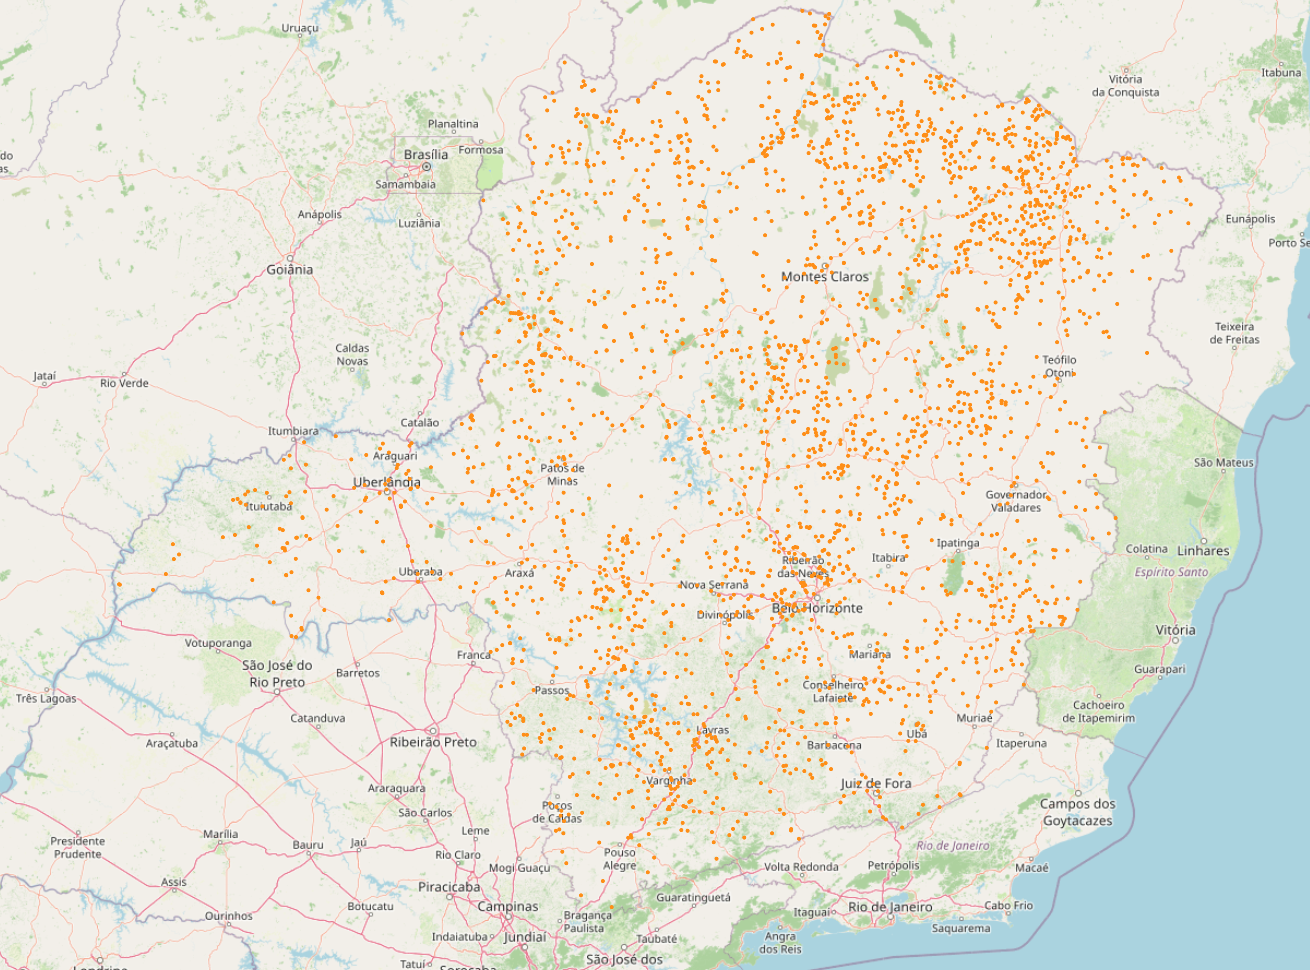
\includegraphics[width=0.7\textwidth]{MapaDeMInas.png}
    \fonte{Autores da pesquisa.}
    \label{fig:mapa}
\end{figure}

Para embasar a robustez, submeteu-se o motor a testes de estresse locais (8 CPUs, 7,5 GiB RAM), variando recursos dos contêineres de consulta (Broker e Historical). A Figura 2 detalha a vazão (QPS) pela concorrência. O perfil de maior alocação sustenta a vazão acima de 2 QPS até concorrência 4. Perfis restritos entram em saturação rapidamente, ratificando a importância do dimensionamento adequado da camada OLAP.

\begin{figure}[H]
    \centering
    \caption{Vazão Analítica do Sistema (QPS) em Função da Concorrência}
    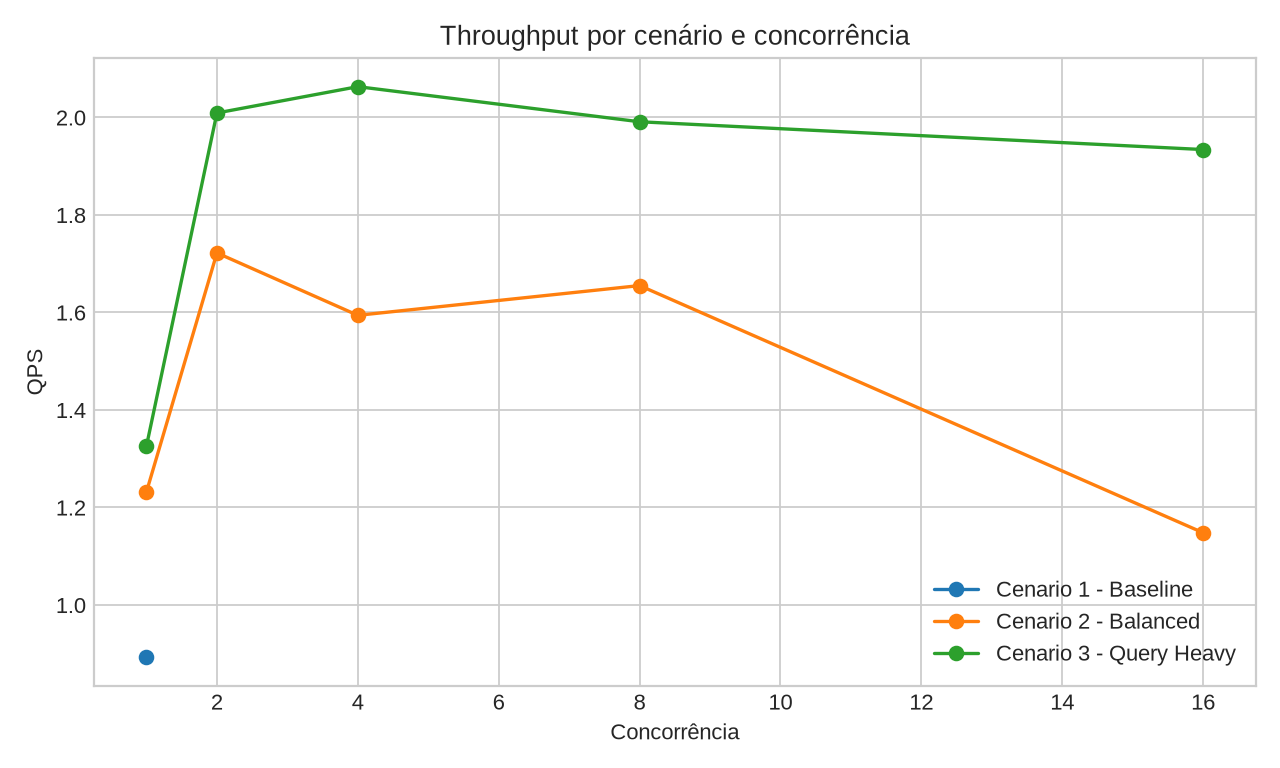
\includegraphics[width=0.9\textwidth]{qps_por_concorrencia.png}
    \fonte{Autores da pesquisa.}
    \label{fig:qps}
\end{figure}

Os resultados comprovam a exequibilidade de transformar registros isolados em inteligência ambiental rápida e coerente. A orquestração garante o cruzamento perene das ameaças contra alvos vulneráveis em tempo hábil para a Defesa Civil.

\section*{Conclusões}

A plataforma CCO-DataOps cumpre seu objetivo técnico ao automatizar a captura, o cruzamento e a indexação de milhares de anomalias térmicas via satélite. O processamento contínuo sobre bases analíticas demonstrou que é viável entregar consultas analíticas de larga escala com vazão superior a duas por segundo sem falhas, cruzando milhões de registros históricos. A validação em Minas Gerais ilustra que a estruturação orientada a eventos, combinada com análises de proximidade para ativos de infraestrutura, é um requisito contemporâneo imperativo, substituindo dados dispersos por respostas rápidas capazes de mitigar os danos catastróficos acarretados por incêndios florestais.

\section*{Agradecimentos}

Expresso minha profunda gratidão à Universidade Federal de Itajubá (UNIFEI) pela infraestrutura concedida para o desenvolvimento desta pesquisa de Iniciação Científica, e ao Conselho Nacional de Desenvolvimento Científico e Tecnológico (CNPq) pelo indispensável apoio financeiro.

\section*{Referências}

AGÊNCIA NACIONAL DE ENERGIA ELÉTRICA (ANEEL). \textbf{Sistema de Informações Geográficas do Setor Elétrico (SIGEL) - Camadas de Transmissão}. Brasília, DF, [2026?]. Disponível em: \url{https://sigel.aneel.gov.br/arcgis/rest/services/PORTAL/}. Acesso em: 11 set. 2026.

BRASIL. Ministério dos Transportes. \textbf{Mapas do Banco de Informações de Transportes (BIT)}. Brasília, DF, [2026?]. Disponível em: \url{https://www.gov.br/transportes/pt-br/pt-br/assuntos/dados-de-transportes/bit/bit-mapas}. Acesso em: 11 set. 2026.

BRUGZ, T. \textbf{GeoData-BR}. Repositório GitHub contendo bases de dados geoespaciais e malhas territoriais do Brasil. [S.l.], 2026. Disponível em: \url{https://github.com/tbrugz/geodata-br}. Acesso em: 11 set. 2026.

ENDSLEY, Mica R. Toward a theory of situation awareness in dynamic systems. \textbf{Human Factors: The Journal of the Human Factors and Ergonomics Society}, v. 37, n. 1, p. 32-64, mar. 1995. DOI: 10.1518/001872095779049543.

ERETH, Julian. DataOps: towards a definition. In: INTERNATIONAL CONFERENCE ON WIRTSCHAFTSINFORMATIK (WI), 13., 2018, St. Gallen. \textbf{Proceedings [...]}. St. Gallen: University of St. Gallen, 2018. p. 104-118.

FUNDAÇÃO NACIONAL DOS POVOS INDÍGENAS (FUNAI). \textbf{Terras Indígenas: Geoprocessamento e Mapas}. Brasília, DF, [2026?]. Disponível em: \url{https://www.gov.br/funai/pt-br/atuacao/terras-indigenas/geoprocessamento-e-mapas}. Acesso em: 11 set. 2026.

GIGLIO, Louis; SCHROEDER, Wilfrid; JUSTICE, Christopher O. The collection 6 MODIS active fire product: Status and first results. \textbf{Remote Sensing of Environment}, v. 174, p. 343-356, mar. 2016.

INSTITUTO NACIONAL DE PESQUISAS ESPACIAIS (INPE). \textbf{Programa Queimadas: Banco de Dados de Queimadas (BDQueimadas)}. São José dos Campos, SP, [2026?]. Disponível em: \url{https://data.inpe.br/queimadas/bdqueimadas/}. Acesso em: 11 set. 2026.

MINISTÉRIO DA SAÚDE (Brasil). DATASUS. \textbf{Cadastro Nacional de Estabelecimentos de Saúde (CNES)}. Brasília, DF, [2026?]. Disponível em: \url{https://cnes.datasus.gov.br/}. Acesso em: 11 set. 2026.

YANG, Fangjin et al. A Fast Column-Store Analytics Database. In: ACM SIGMOD INTERNATIONAL CONFERENCE ON MANAGEMENT OF DATA, 2014, Snowbird. \textbf{Proceedings [...]}. Snowbird: ACM, 2014. p. 157-168.


\end{document}
